\documentclass{beamer}
\usepackage[russian]{babel}
\begin{document}
\begin{frame}{
\includegraphics[width=4em]{picture_logo.png} Перевод из одной СС в другую. Пример 2}
\begin{center}
    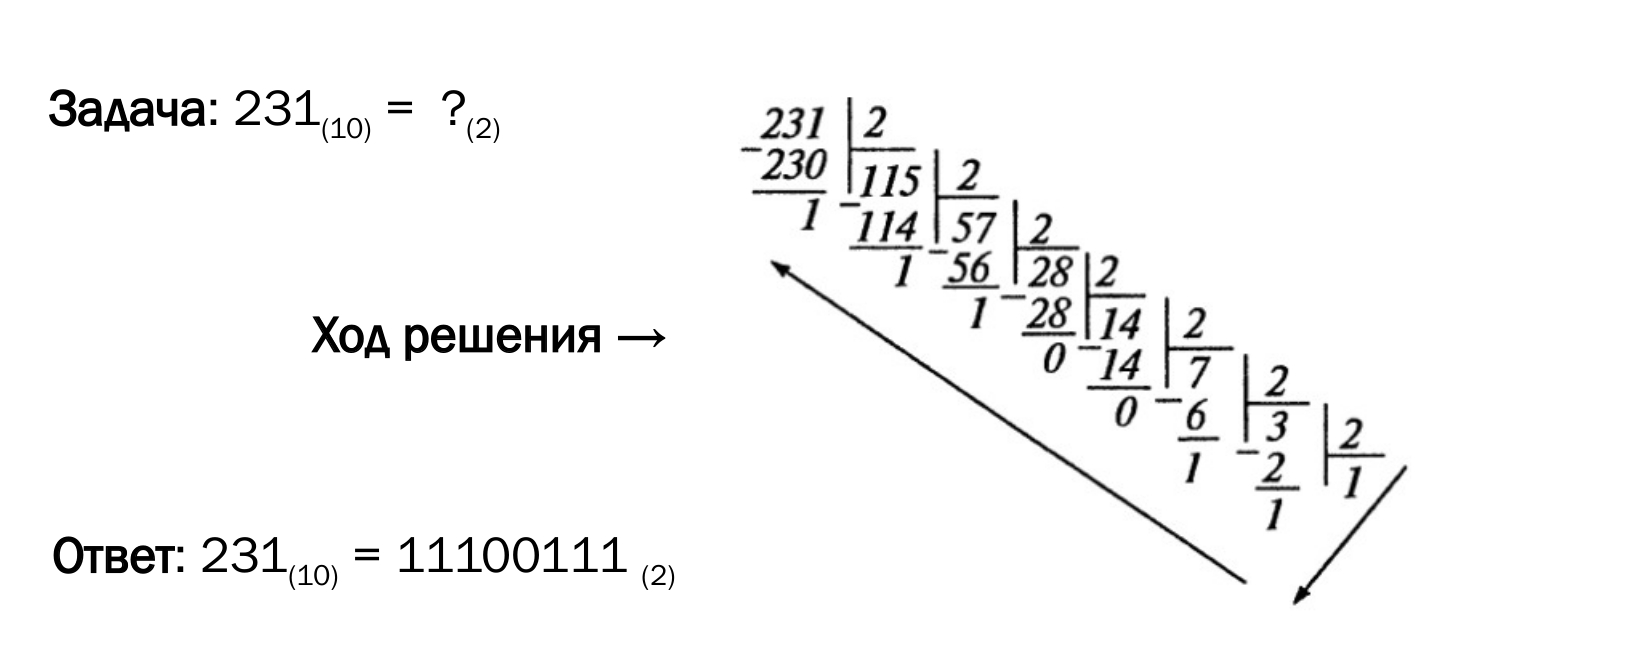
\includegraphics[width=\columnwidth]{26.png}
\end{center}
\end{frame}
\begin{frame}{
\includegraphics[width=4em]{picture_logo.png} Перевод из одной СС в другую. Пример 4}

\begin{center}
    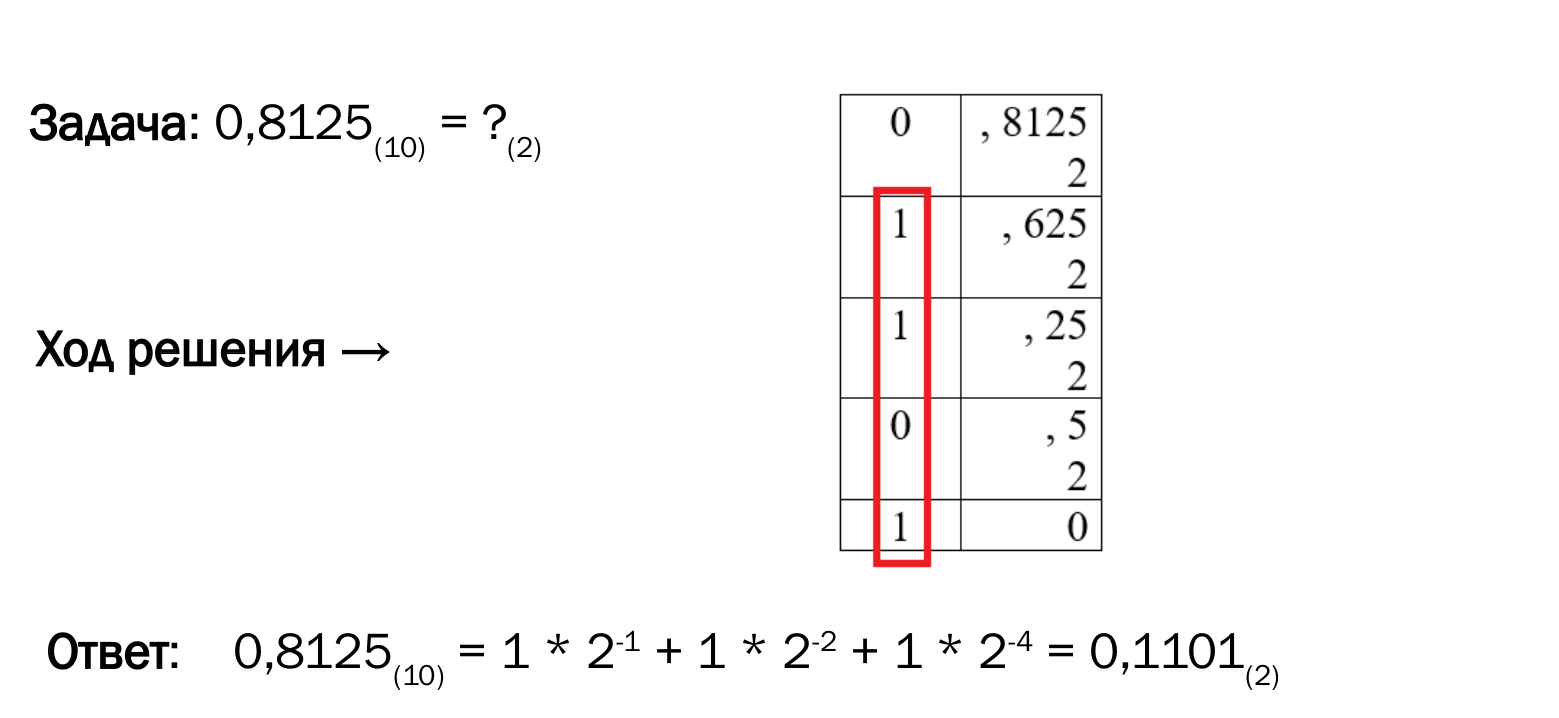
\includegraphics[width=\columnwidth]{28.png}
\end{center}
\textbf{Ответ:} $0,8125_{(10)} = 1 * 2^{-1} + 1 * 2^{-2} + 1 * 2^{-4} = 0,1101_2$
\end{frame}
\begin{frame}{
\includegraphics[width=4em]{picture_logo.png} Преобразование из CC-\textit{N} в CC-$N^k$  и обратно}
\textcolor[RGB]{57, 255, 20}{Из CC-\textit{N} в CC-$N^k$}\\
\begin{itemize}
  \item дополнить число, записанное в СС с основанием $N$, незначащими нулями так, чтобы количество цифр было кратно $k$;
  \item разбить полученное число на группы по $k$ цифр, начиная от нуля;
  \item заменить каждую такую группу эквивалентным числом, записанным в СС с основанием $N^k$.
\end{itemize}

Задача: $1020101_{(3)} = ?_{(27)}$\\
Решение: $1020101_{(3)} = 001\hphantom1020\hphantom1101_{(3)} = 16A?_{(27)}$\\
\vspace{1em}
\textcolor[RGB]{57, 255, 20}{Из CC-$N^k$ в CC-\textit{N}}\\
\begin{itemize}
    \item  заменить каждую цифру числа, записанного в CC с основанием $N^k$, эквивалентным набором из $k$ цифр CC с основанием $N$.
\end{itemize}
Задача: $2345_{(125)} = ?_{(5)}$\\
Решение: $2345_{(3)} = 002\hphantom1003\hphantom1004\hphantom1010_{(5)} = 2003004010_{(5)}$\\
\end{frame}

\begin{frame}{\includegraphics[width=4em]{picture_log.png} Оптимальная система счисления}
\begin{center}
    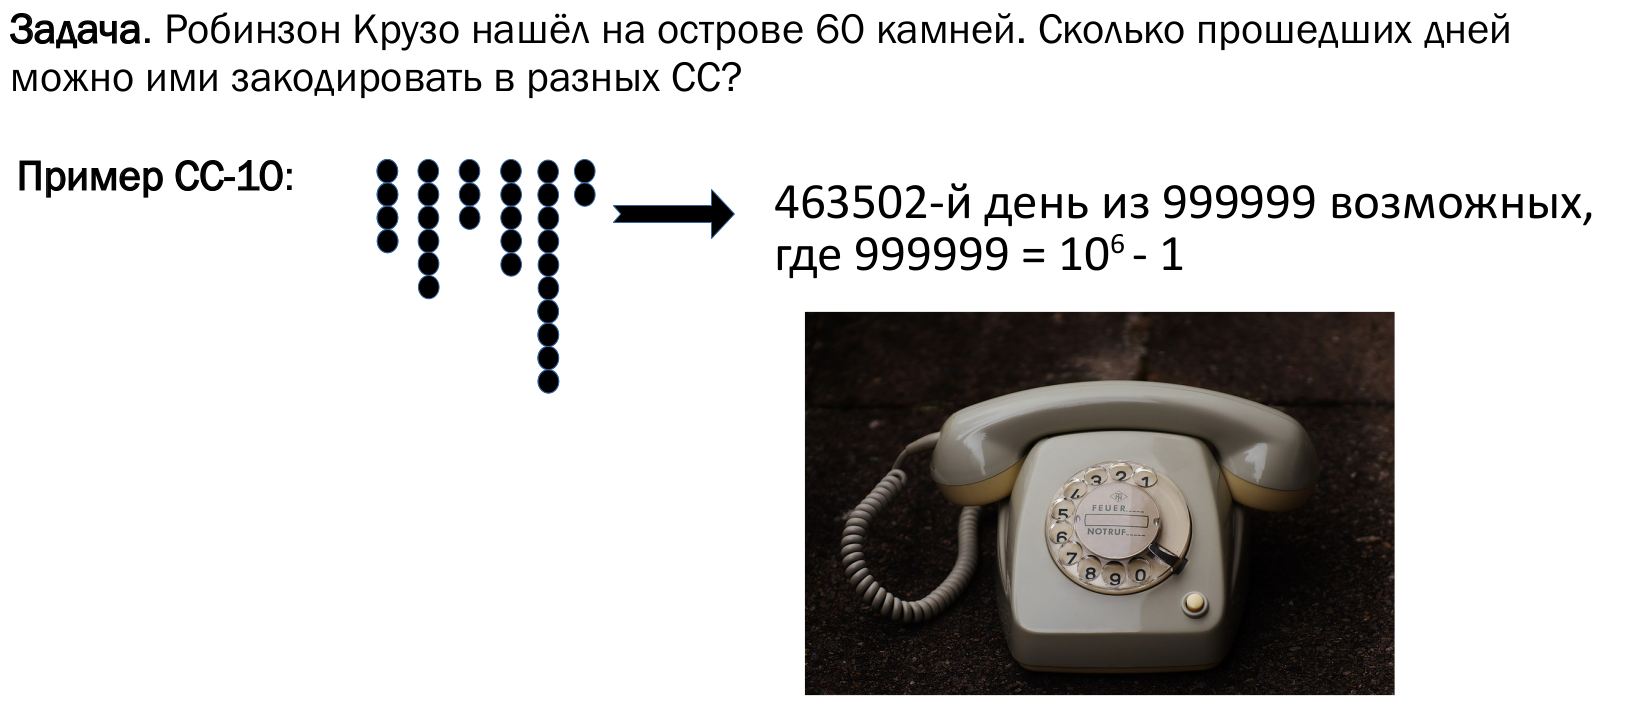
\includegraphics[width=\columnwidth]{33.png}
\end{center}
\end{frame}

\begin{frame}{
\includegraphics[width=4em]{picture_logo.png} Оптимальная система счисления (2)}
\begin{center}
    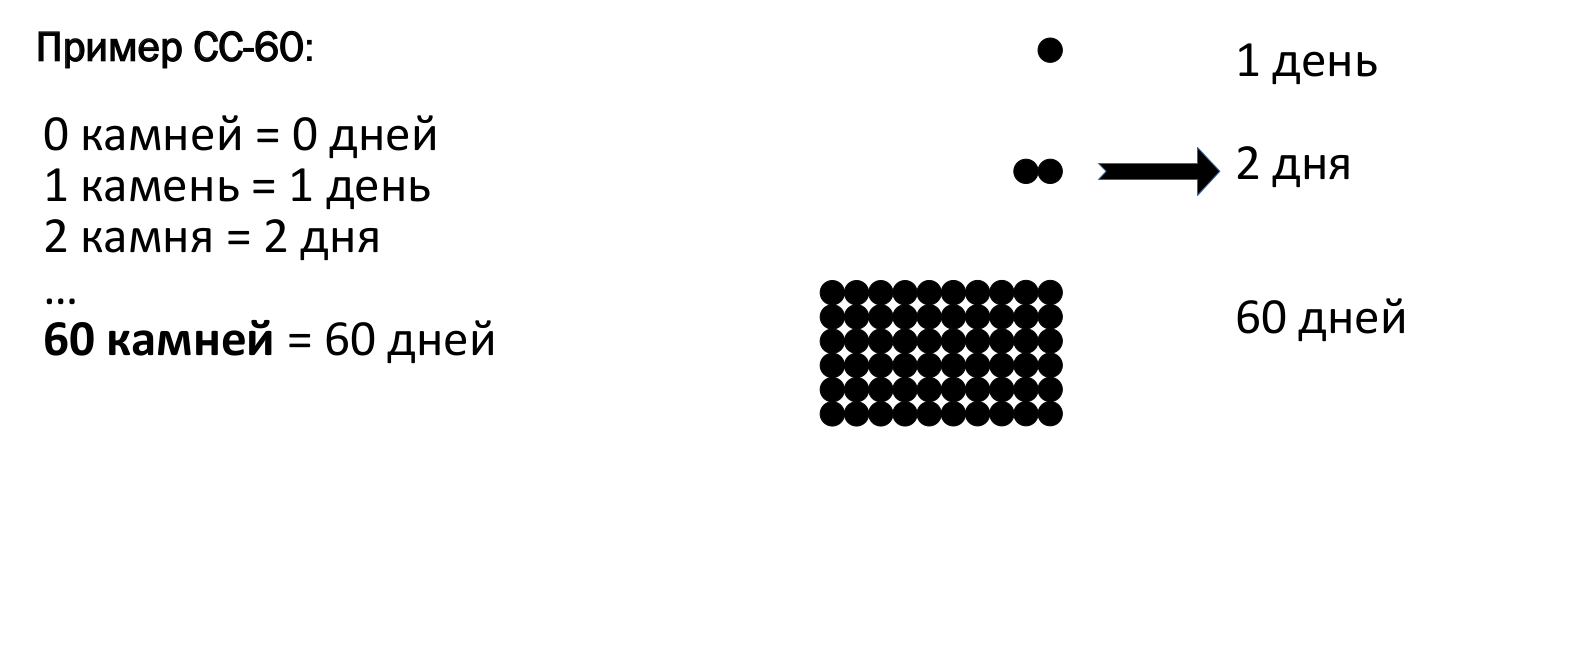
\includegraphics[width=\columnwidth]{34.png}
\end{center}
\end{frame}

\end{document}
